\section{Fault detection and isolation on steel plates}

\begin{frame}
	\frametitle{Dataset description}
	The steel plates faults dataset comes from research by Semeion, Research Center of Sciences of Communication. The aim of the research was to correctly classify the type of surface defects in stainless steel plates. Below is some information about the dataset:
	\begin{itemize}
		\item number of fault classes: $6 + 1$ (no faults);
		\item number of attributes: $27$;
		\item number of instances: $1941$;
		\item absence of missing values.
	\end{itemize}
	Unfortunately, no further details on the covariates are available.
\end{frame}

\begin{frame}
	\frametitle{Preliminary analysis}
	\begin{figure}
		\centering
		\begin{subfigure}[b]{0.49\textwidth}
			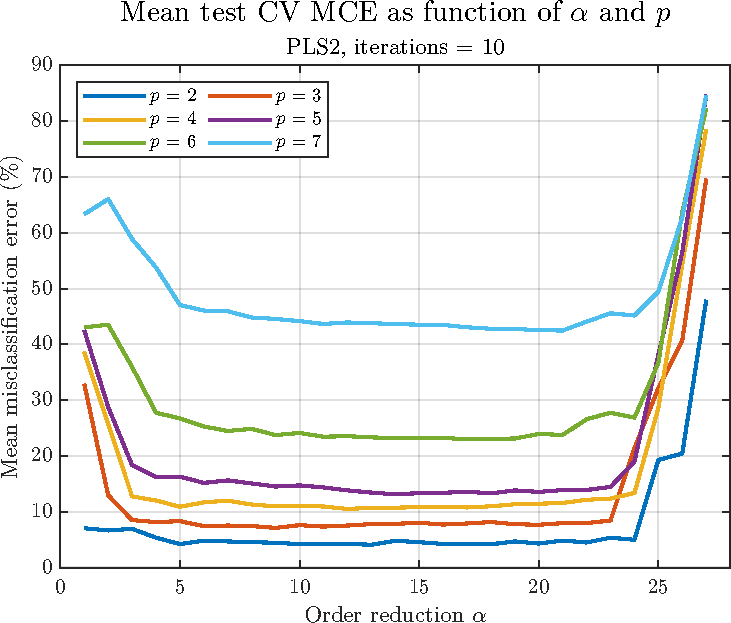
\includegraphics[width=\textwidth]{Images/trend_alpha_p_PLS2.pdf}
		\end{subfigure}
		\hfill
		\begin{subfigure}[b]{0.49\textwidth}
			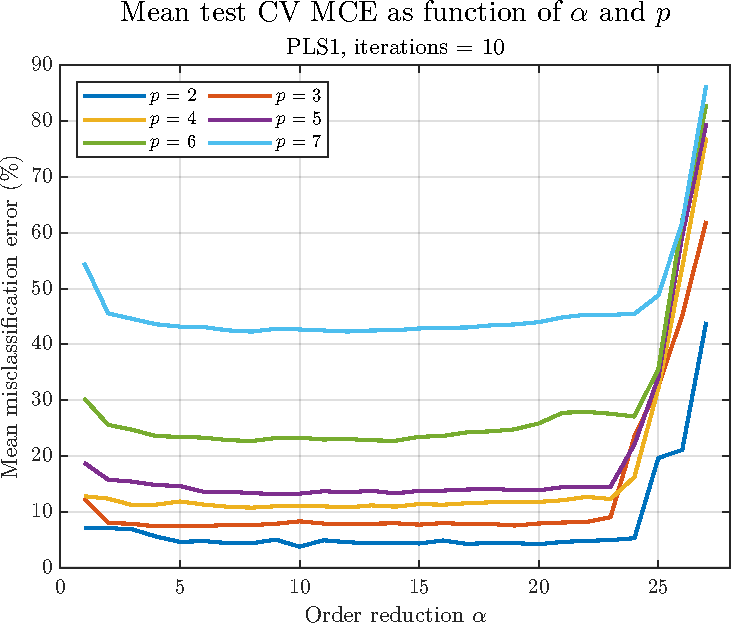
\includegraphics[width=\textwidth]{Images/trend_alpha_p_PLS1.pdf}
		\end{subfigure}
	\end{figure}
	As the number of fault classes \textit{p} taken into consideration increases, the mean test CV MCE also increases. Both algorithms show a similar behaviour in case of overfitting, while PLS1 underfits less than PLS2. 
\end{frame}

\begin{frame}
	\frametitle{Methodology}
	To reduce the dependency on a specific dataset randomization during the $10$-folds cross-validation, we decided to iterate this procedure $n$ times ($10$ in preliminary analysis). We used the CV technique to make inference on the model parameters, especially to choose the best model reduction $\alpha$.\\ As we can see from graphs in the previous frame, with $p = 5$ we obtain a model that is a good compromise between complexity and cross-validation performances, therefore we decided to make our in-depth analysis with this model.
\end{frame}

\begin{frame}
	\frametitle{In-depth analysis with $p = 5$}
	\begin{figure}
		\centering
		\begin{subfigure}[b]{0.49\textwidth}
			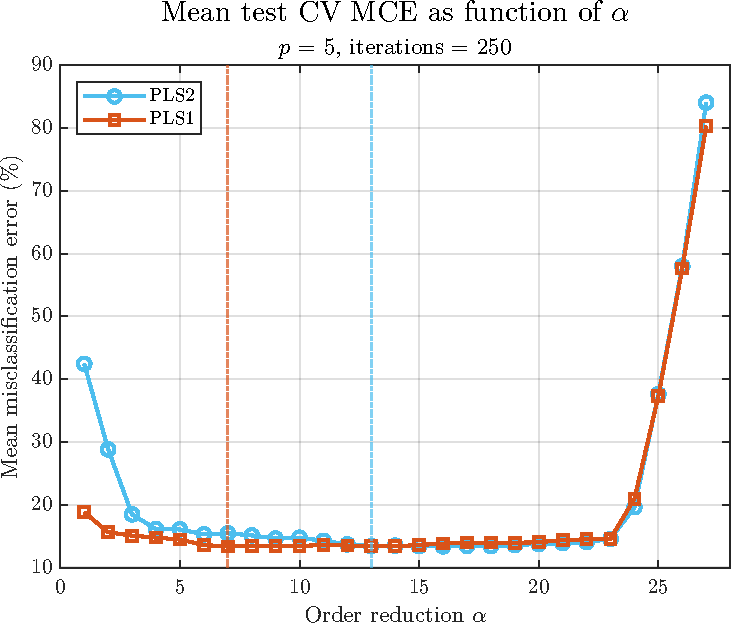
\includegraphics[width=\textwidth]{Images/trend_alpha_5.pdf}
		\end{subfigure}
		\hfill
		\begin{subfigure}[b]{0.49\textwidth}
			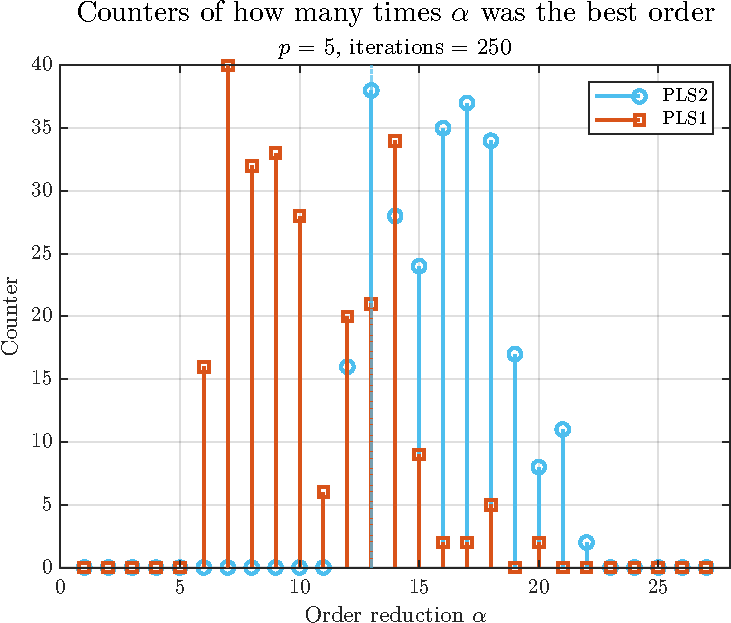
\includegraphics[width=\textwidth]{Images/counters_alpha_5.pdf}
		\end{subfigure}
	\end{figure}
	In right figure we can note that PLS2 tends to advise more complex models than PLS1. This behaviour is confirmed by left graph: PLS2 goes underfit faster than the other algorithm
\end{frame}

\begin{frame}
	\begin{figure}
		\centering
		\begin{subfigure}[b]{0.60\textwidth}
			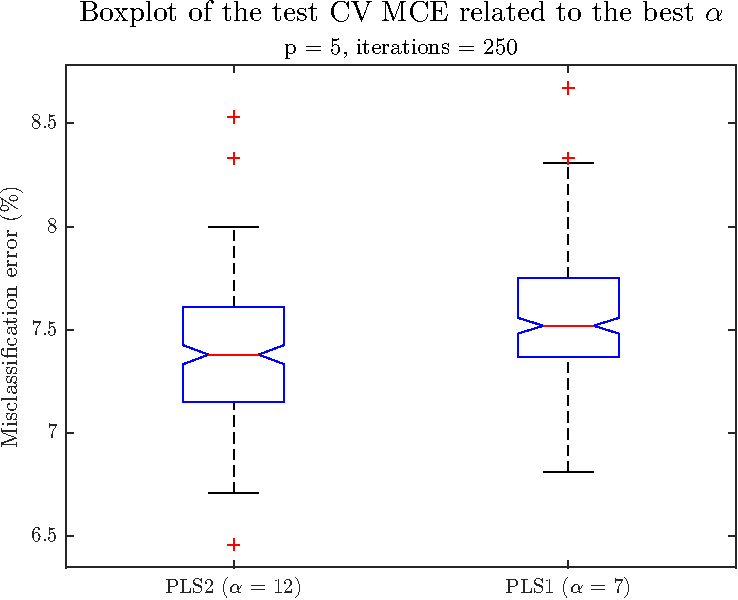
\includegraphics[width=\textwidth]{Images/box_alpha_5.pdf}
		\end{subfigure}
	\end{figure}
	Although PLS1 performs slightly better on average than PLS2, we decided to use the latter one for the following analyses because it is the model with the shortest estimation time.
\end{frame}

\begin{frame}
	\frametitle{Validation $70-30$ of the PLS2 model with $\alpha = 13$}
	\begin{figure}
		\begin{subfigure}[b]{0.49\textwidth}
			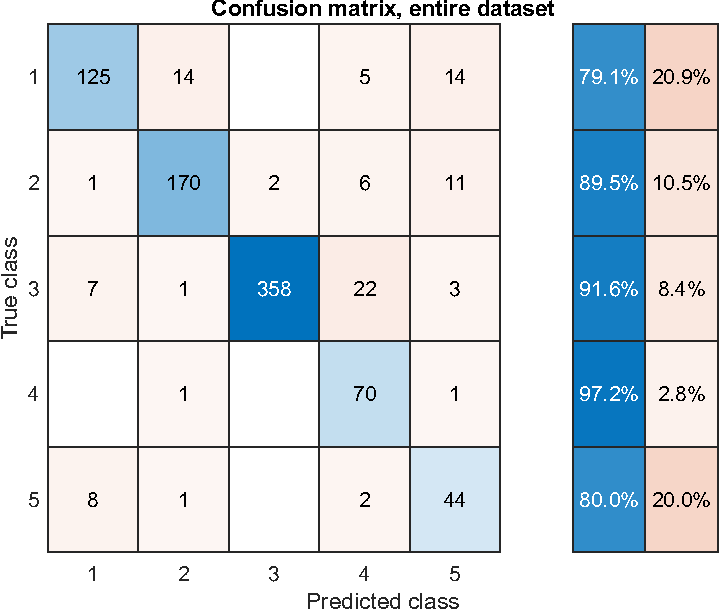
\includegraphics[width=\textwidth]{Images/confusion_all_5_PLS2.pdf}
		\end{subfigure}
		\hfill
		\begin{subfigure}[b]{0.49\textwidth}
			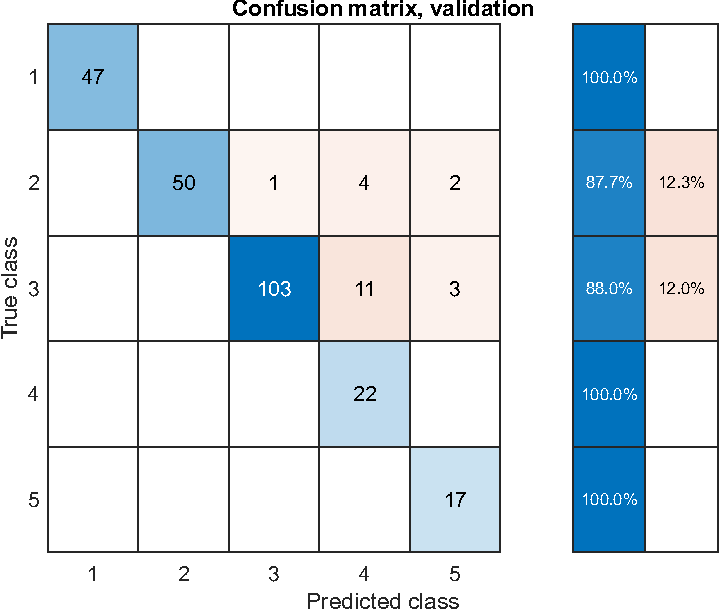
\includegraphics[width=\textwidth]{Images/confusion_val_5_PLS2.pdf}
		\end{subfigure}
	\end{figure}
	We can see that in validation there is a natural decrease in the predictive capabilities of the model. In particular, the fault classes on which PLS2 struggles the most are classes $1$ and $5$.
\end{frame}

\begin{frame}
	\frametitle{Score matrix $T$ with $\alpha = 1$, $2$ and $3$}
	\begin{figure}
		\begin{subfigure}[b]{0.49\textwidth}
			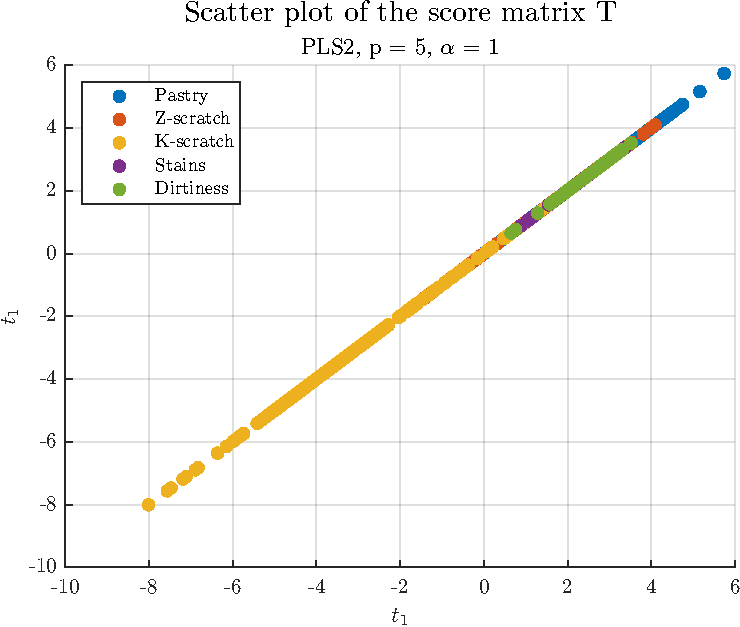
\includegraphics[width=\textwidth]{Images/scatter_T_a1_p5.pdf}
		\end{subfigure}
		\hfill
		\begin{subfigure}[b]{0.49\textwidth}
			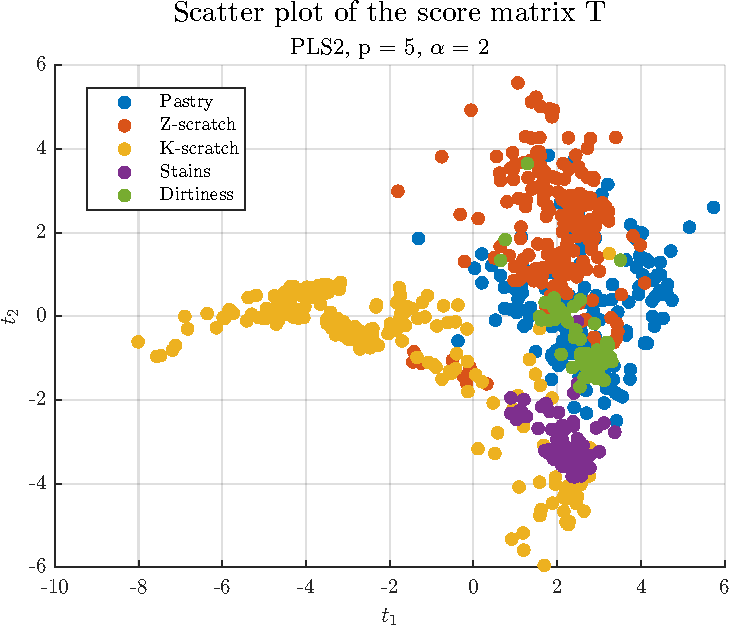
\includegraphics[width=\textwidth]{Images/scatter_T_a2_p5.pdf}
		\end{subfigure}
	\end{figure}
\end{frame}

\begin{frame}
	\begin{figure}
		\begin{subfigure}[b]{0.60\textwidth}
			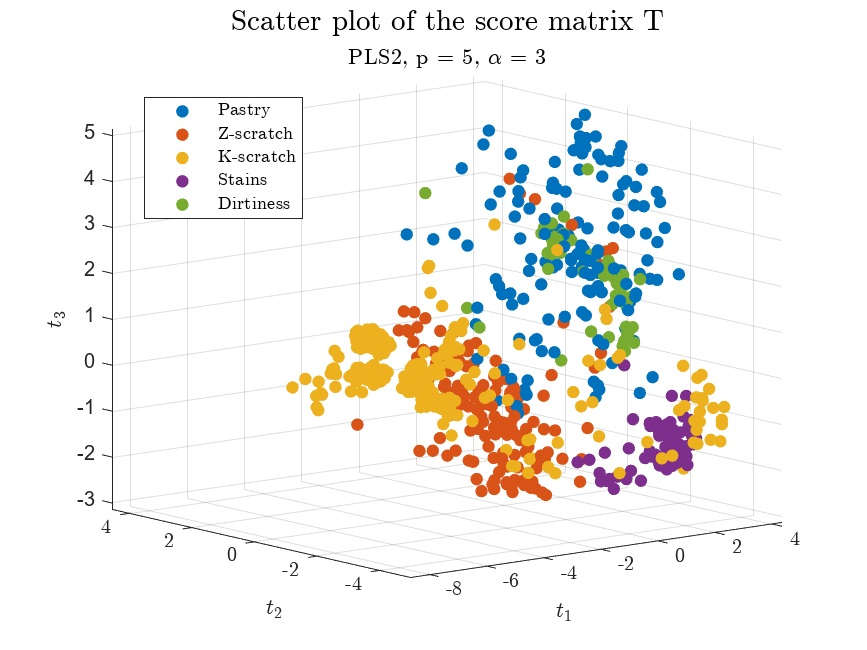
\includegraphics[width=\textwidth]{Images/scatter_T_a3_p5.pdf}
		\end{subfigure}
	\end{figure}
	\begin{table}
		\centering
		\renewcommand\arraystretch{1.3}
		\begin{tabular}{c|c|c|c|c|c|c}
			\hline
			$\boldsymbol{\alpha}$ & \textbf{Pastry} & \textbf{Z-scratch} & \textbf{K-scratch} & \textbf{Stains} & \textbf{Dirtiness} & \textbf{Average}\\
			\hline
			\num{1} & $1.27\%$ & $100\%$ & $11.76\%$ & $100\%$ & $100\%$ & $42.15\%$ \\
			\num{2} & $77.85\%$ & $8.95\%$ & $12.53\%$ & $1.39\%$ & $100\%$ & $28.29\%$ \\
			\num{3} & $15.82\%$ & $10\%$ & $14.58\%$ & $1.39\%$ & $100\%$ & $18.13\%$ \\ 
			\hline
		\end{tabular}
	\end{table}
\end{frame}